%%%%%%%%%%%%%%%%%%%%%%%%%%%%%%%%%%%%%%%%%
% Beamer Presentation
% LaTeX Template
% Version 1.0 (10/11/12)
%
% This template has been downloaded from:
% http://www.LaTeXTemplates.com
%
% License:
% CC BY-NC-SA 3.0 (http://creativecommons.org/licenses/by-nc-sa/3.0/)
%
%%%%%%%%%%%%%%%%%%%%%%%%%%%%%%%%%%%%%%%%%

%----------------------------------------------------------------------------------------
%	PACKAGES AND THEMES
%----------------------------------------------------------------------------------------

\documentclass{beamer}

\mode<presentation> {

% The Beamer class comes with a number of default slide themes
% which change the colors and layouts of slides. Below this is a list
% of all the themes, uncomment each in turn to see what they look like.

%\usetheme{default}
%\usetheme{AnnArbor}
%\usetheme{Antibes}
%\usetheme{Bergen}
%\usetheme{Berkeley}
%\usetheme{Berlin}
%\usetheme{Boadilla}
%\usetheme{CambridgeUS}
%\usetheme{Copenhagen}
%\usetheme{Darmstadt}
%\usetheme{Dresden}
%\usetheme{Frankfurt}
%\usetheme{Goettingen}
%\usetheme{Hannover}
%\usetheme{Ilmenau}
%\usetheme{JuanLesPins}
%\usetheme{Luebeck}
\usetheme{Madrid}
%\usetheme{Malmoe}
%\usetheme{Marburg}
%\usetheme{Montpellier}
%\usetheme{PaloAlto}
%\usetheme{Pittsburgh}
%\usetheme{Rochester}
%\usetheme{Singapore}
%\usetheme{Szeged}
%\usetheme{Warsaw}

% As well as themes, the Beamer class has a number of color themes
% for any slide theme. Uncomment each of these in turn to see how it
% changes the colors of your current slide theme.

%\usecolortheme{albatross}
%\usecolortheme{beaver}
%\usecolortheme{beetle}
%\usecolortheme{crane}
%\usecolortheme{dolphin}
%\usecolortheme{dove}
%\usecolortheme{fly}
%\usecolortheme{lily}
%\usecolortheme{orchid}
%\usecolortheme{rose}
%\usecolortheme{seagull}
%\usecolortheme{seahorse}
%\usecolortheme{whale}
%\usecolortheme{wolverine}

%\setbeamertemplate{footline} % To remove the footer line in all slides uncomment this line
%\setbeamertemplate{footline}[page number] % To replace the footer line in all slides with a simple slide count uncomment this line

%\setbeamertemplate{navigation symbols}{} % To remove the navigation symbols from the bottom of all slides uncomment this line
}

\usepackage{graphicx} % Allows including images
\usepackage{booktabs} % Allows the use of \toprule, \midrule and \bottomrule in tables
\usepackage[utf8]{inputenc}

%----------------------------------------------------------------------------------------
%	TITLE PAGE
%----------------------------------------------------------------------------------------

\title[]{Análisis evolutivo de insectos transgénicos de la especie \textit{Rhodnius prolixus} en el tratamiento de la enfermedad de Chagas } % The short title appears at the bottom of every slide, the full title is only on the title page

\author{Nancy Ruiz-Sergio Hernández} % Your name
\institute[Uniandes] % Your institution as it will appear on the bottom of every slide, may be shorthand to save space
{
Universidad de los Andes \\ % Your institution for the title page
 % Your email address
}
\date{\today} % Date, can be changed to a custom date

\begin{document}

\begin{frame}
\titlepage % Print the title page as the first slide
\end{frame}

\begin{frame}
\frametitle{General} % Table of contents slide, comment this block out to remove it
\tableofcontents % Throughout your presentation, if you choose to use \section{} and \subsection{} commands, these will automatically be printed on this slide as an overview of your presentation
\end{frame}

%----------------------------------------------------------------------------------------
%	PRESENTATION SLIDES
%----------------------------------------------------------------------------------------

%------------------------------------------------
\section{Introducción} % Sections can be created in order to organize your presentation into discrete blocks, all sections and subsections are automatically printed in the table of contents as an overview of the talk
%------------------------------------------------




















%------------------------------------------------

\begin{frame}
\frametitle{Introducción}
\begin{columns}[c] % The "c" option specifies centered vertical alignment while the "t" option is used for top vertical alignment
\column{.35\textwidth} % Left column and width
\begin{itemize}
\item Enfermedad de Chagas
\item Tripanosoma \textit{cruzi}
\item Vector Rhodnius \textit{prolixius}
\end{itemize}
\column{.55\textwidth} % Right column and width
\begin{figure}[ht!]
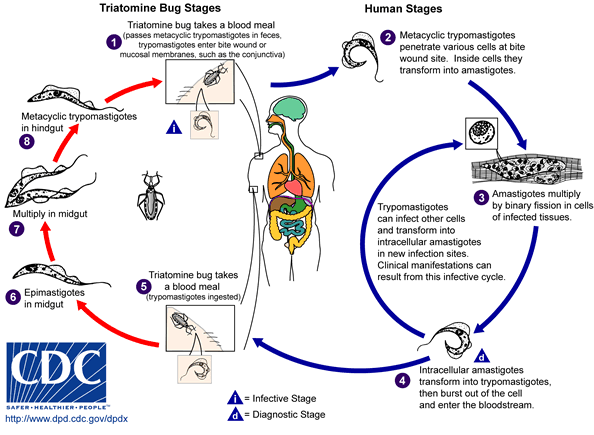
\includegraphics[scale=0.45]{Trypanosoma_cruzi_LifeCycle.png} 
\caption{Ciclo de vida de T.\textit{cruzi}}
\end{figure}  
\end{columns}
\end{frame}

%------------------------------------------------

\begin{frame}
\frametitle{Paratránsgenesis}
\begin{columns}[c] % The "c" option specifies centered vertical alignment while the "t" option is used for top vertical alignment
\column{.35\textwidth} % Left column and width
\begin{itemize}
\item Inserción de un plásmido pRrMDWK6 en una bacteria simbionte del vector \textit{R.prolixus}
\end{itemize}
\begin{figure}[ht!]
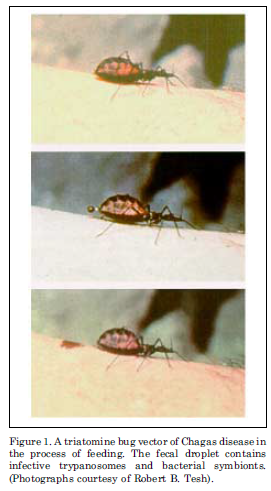
\includegraphics[scale=0.3]{insectos2.PNG} 
\caption{Idea General}
\end{figure} 
\column{.55\textwidth} % Right column and width
\begin{figure}[ht!]
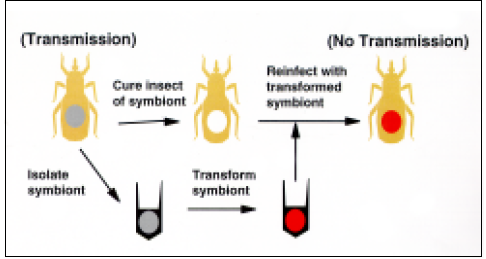
\includegraphics[scale=0.55]{insectos.png} 
\caption{Idea General}
\end{figure}


\end{columns}
\end{frame}

%------------------------------------------------
\section{Protocolo y diseño experimental}

\begin{frame}
\frametitle{Protocolo y Diseño Experimental}
\begin{columns}[c] % The "c" option specifies centered vertical alignment while the "t" option is used for top vertical alignment
\column{.35\textwidth} % Left column and width
\begin{itemize}
\item Cultivo y Transformación de las bacterias
\item Plásmido pRrMDWK6
\item Transformación de los vectores
\item Reconocimiento del anticuerpo
\end{itemize}
\column{.55\textwidth} % Right column and width
\begin{figure}[ht!]
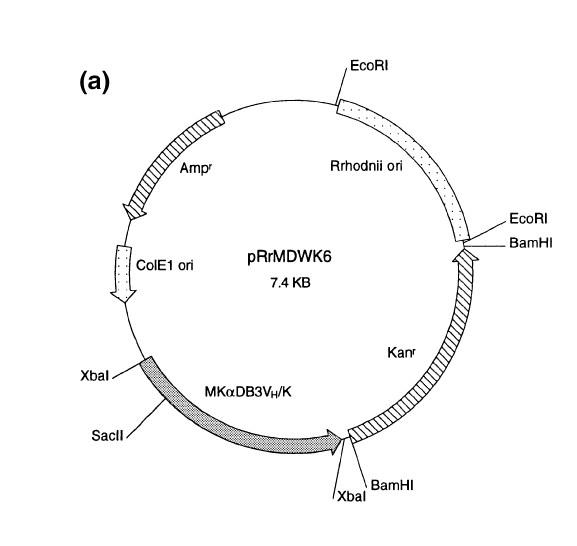
\includegraphics[scale=0.25]{plasmido+.PNG} 
\caption{Plásmido pRrMDWK6}
\end{figure} 
\begin{figure}[ht!]
\vspace*{-1cm}
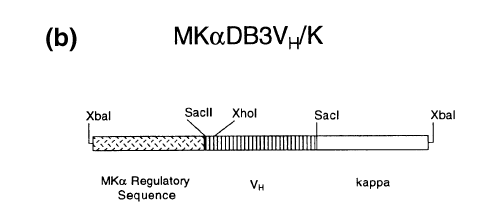
\includegraphics[scale=0.3]{cassete.PNG} 
\caption{Circuito}
\end{figure} 
\end{columns}
\end{frame}

%------------------------------------------------
\section{Modelo evolutivo}


\begin{frame}
\frametitle{Modelo evolutivo}
\begin{columns}[c] % The "c" option specifies centered vertical alignment while the "t" option is used for top vertical alignment
\column{.5\textwidth} % Left column and width
\begin{itemize}
\item Escogencia de las constantes
\item Modelo de Moran
\item Algoritmo de Guillespie
\item Exhaustivo
\item Aproximaciones (plásmido R1)
\item Poblaciones con R.\textit{rhodnii}
\end{itemize}
\column{.5\textwidth} % Right column and width


\begin{figure}[ht!]
\vspace*{-1cm}
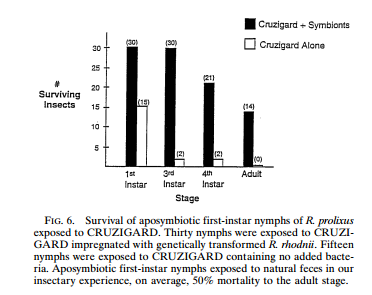
\includegraphics[scale=0.4]{supervivencia.png} 
\end{figure}

\begin{figure}[ht!]
\vspace*{-1cm}
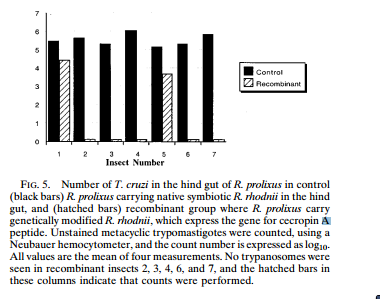
\includegraphics[scale=0.4]{super_parasitos.png} 
\end{figure}




\end{columns}
\end{frame}

%------------------------------------------------

\begin{frame}
\frametitle{Modelo de Moran}
\begin{columns}[c] % The "c" option specifies centered vertical alignment while the "t" option is used for top vertical alignment
\column{.55\textwidth} % Left column and width
\begin{figure}[ht!]
\vspace*{-1cm}
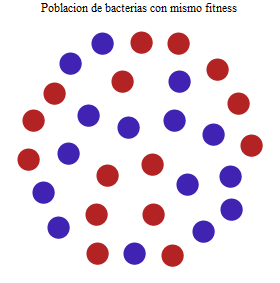
\includegraphics[scale=0.5]{same_fitness.png} 
\caption{Modelo de Moran}
\end{figure} 
\column{.45\textwidth} % Right column and width
\begin{itemize}
\item Proceso estocástico que describe poblaciones finitas.
\item Fitness Relativo
\item Implementado en Mathematica
\end{itemize}
\end{columns}
\end{frame}

%------------------------------------------------

\begin{frame}
\frametitle{Modelo de Moran}
\[ T_{i \rightarrow i+1}= \frac{i f_{A} \left(i\right)}{i f_{A}\left(i\right)+ \left(N-i\right) f_{B}\left(i\right)} \frac{N-i}{N}\]

\[ T_{i \rightarrow i-1}= \frac{\left( N-i \right) f_{B} \left(i\right) }{i f_{A}\left(i\right)+ \left(N-i\right) f_{B}\left(i\right)} \frac{i}{N}\]

\[ T_{i \rightarrow i}= 1 - T_{i \rightarrow i+1} - T_{i \rightarrow i-1} \]
\end{frame}

%------------------------------------------------

%------------------------------------------------

\begin{frame}
\frametitle{Resultados - Modelo de Moran}
\begin{columns}[c] % The "c" option specifies centered vertical alignment while the "t" option is used for top vertical alignment
\column{.5\textwidth} % Left column and width
\begin{figure}[ht!]
\vspace*{-1cm}
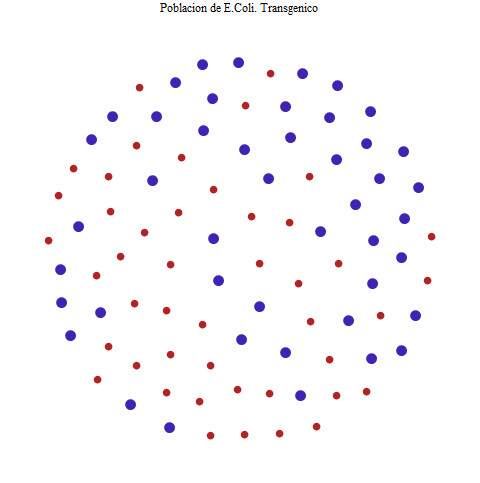
\includegraphics[scale=0.16]{ecoli_moran_1.png} 
\caption{Primera Generación}
\end{figure} 
\begin{figure}[ht!]
\vspace*{-1cm}
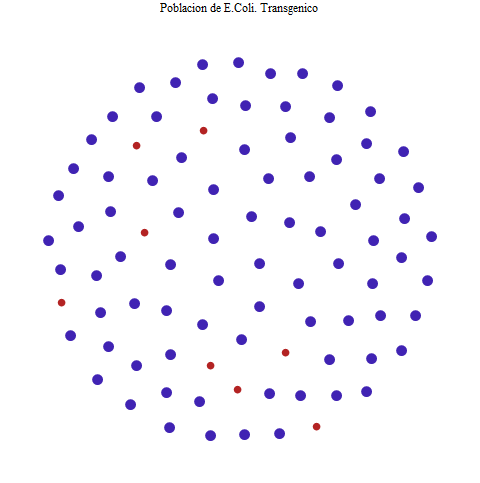
\includegraphics[scale=0.16]{ecoli_moran_339.png} 
\caption{Generación 339}
\end{figure} 
\column{.5\textwidth} % Right column and width
\begin{figure}[ht!]
\vspace*{-1cm}
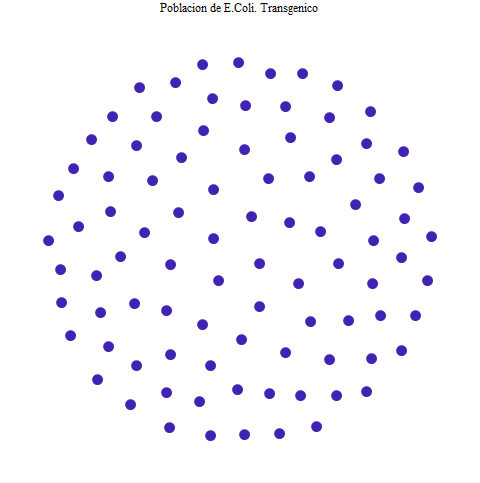
\includegraphics[scale=0.2]{ecoli_moran_576.png} 
\caption{Generación final, 576}
\end{figure} 
\begin{figure}[ht!]
\vspace*{-1cm}
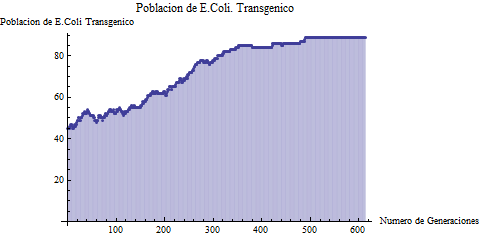
\includegraphics[scale=0.2]{poblacion_ecoli_trans.png} 
\caption{Evolución de la población de E.\textit{coli}}
\end{figure} 
\end{columns}
\end{frame}

%------------------------------------------------

%------------------------------------------------

\begin{frame}
\frametitle{Resultados - Algoritmo de Gillepsie}

\begin{figure}[ht!]
\vspace*{-1cm}
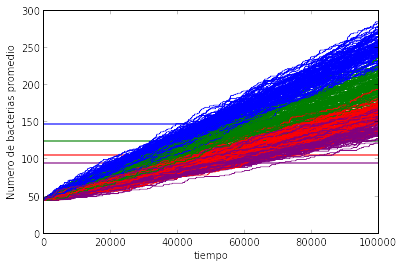
\includegraphics[scale=0.65]{todasLasCorridas.png} 
\caption{Evolución de las poblaciones}
\end{figure} 

\end{frame}

%------------------------------------------------
\section{Consideraciones éticas}

\begin{frame}
\frametitle{Consideraciones éticas}

\begin{itemize}
\item Consecuencias ecológicas y regulación
\item Dominancia de organismos no transformados
\item Transferencia horizontal de genes
\begin{figure}[ht!]
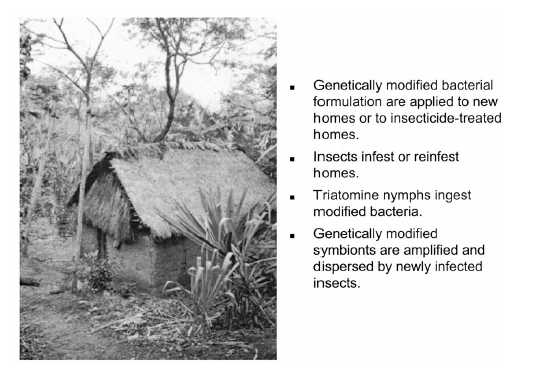
\includegraphics[scale=0.4]{casa.PNG} 

\end{figure} 

\end{itemize}
\end{frame}

%------------------------------------------------
\section{Dificultades generales}

\begin{frame}
\frametitle{Dificultades generales}
\begin{columns}[c] % The "c" option specifies centered vertical alignment while the "t" option is used for top vertical alignment
\column{.5\textwidth} % Left column and width
\begin{itemize}
\item Evolución del proyecto
\item Escogencia de las constantes
\item Modelo
\end{itemize}
\begin{figure}[ht!]
\vspace*{-0.2cm}
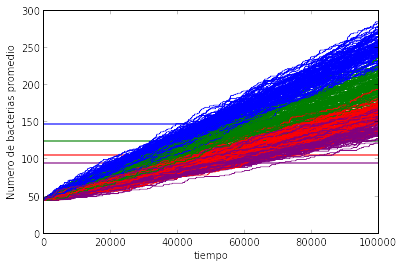
\includegraphics[scale=0.2]{todasLasCorridas.png} 
\caption{Evolución de las poblaciones}
\end{figure} 
\column{.5\textwidth} % Right column and width
\begin{figure}[ht!]
\vspace*{-1cm}
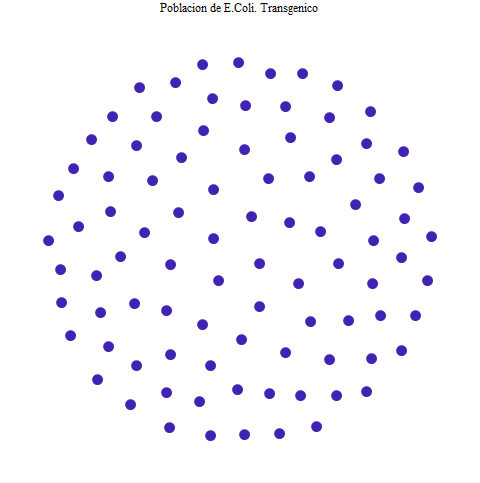
\includegraphics[scale=0.2]{ecoli_moran_576.png} 
\caption{Generación final, 576}
\end{figure} 
\begin{figure}[ht!]
\vspace*{-1cm}
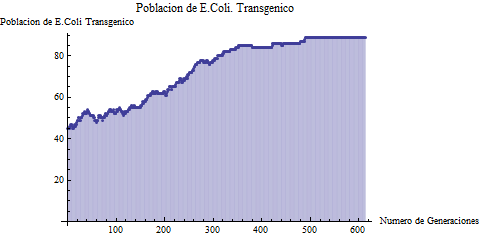
\includegraphics[scale=0.2]{poblacion_ecoli_trans.png} 
\caption{Evolución de la población de E.\textit{coli}}
\end{figure} 
\end{columns}
\end{frame}

%--------------------------------

\section{Conclusiones}



\begin{frame}
\frametitle{Conclusiones}
\begin{itemize}
\item De nuestro análisis evolutivo es posible concluir que la bacteria que presentó el mayor fitness y por ende la que mejor pudo adaptarse a la inserción del plásmido para la eliminación de bacterias fue E.Coli, seguida de Salmonella y finalmente R.rhodnii
\item No fue posible realizar un modelo sofisticado debido a la imposibilidad de encontrar las constantes de producción y degradación de anticuerpos.
\item Para realizar adecuadamente este análisis es necesaria una parte experimental en la que se pueda medir el fitness de las bacterias con el plásmido y la tasa de degradación y producción de anticuerpos.
\end{itemize}


\end{frame}

%------------------------------------------------

%------------------------------------------------

\section{Referencias}
%------------------------------------------------




%------------------------------------------------

\begin{frame}
\frametitle{References}
\scriptsize{
\begin{thebibliography}{99} % Beamer does not support BibTeX so references must be inserted manually as below
\bibitem[Hurwitz, 2011]{p1} Hurwitz, Fieck (2011)
\newblock Paratransgenic control of vector borne diseases

\bibitem[Eichler, 2002]{p1} Eichler, Schaub (2002)
\newblock Development of symbionts in triatomine bugs and the effects of infections with trypanosomatids

\bibitem[Lenski, 1998]{p1} Lenski, Mongold (1998)
\newblock Evolution of competitive fitness in experimental populations of E. coli: what makes one genotype a better competitor than another?

\bibitem[Dionisio, 2005]{p1} Dionisio, Conceicao (2005)
\newblock The evolution of a conjugative plasmid and its ability to increase bacterial fitness

\bibitem[Dotson, 2003]{p1} Dotson, Plikaytis, Durvasula (2003)
\newblock Transformation of Rhodococcus rhodnii, a symbiont of the Chagas disease vector Rhodnius prolixus, with integrative elements of the L1 mycobacteriophage

\bibitem[He, 1995]{p1} He, Hamon, Liu (1995)
\newblock Functional expression of a single-chain anti-progesterone antibody fragment in the cytoplasm of a mutant Escherichia coli

\bibitem[Matsuo, 1990]{p1} Matsuo, Yamaguchi, Yamazaki (1990)
\newblock Establishment of a foreign antigen secretion system in mycobacteria

\end{thebibliography}
}
\end{frame}

%------------------------------------------------

\begin{frame}
\Huge{\centerline{Gracias!}}
\end{frame}

%----------------------------------------------------------------------------------------

\end{document}